\message{ !name(manuscript.tex)}\documentclass{article}
\usepackage{amssymb}
\usepackage{bbm}
\usepackage{graphicx}
\usepackage[margin=1in]{geometry}
\newcommand{\x}X
\newcommand{\p}p
\newcommand{\n}n
\newcommand{\m}m
\renewcommand{\c}c
\begin{document}

\message{ !name(manuscript.tex) !offset(-3) }



Exact, nonparametric estimation of incidence for repeated measurements


\section{Method}

\subsection{Data}
The data are $n$ IID vectors of length
$m$ of binary values, 
$(\x_{11},\x_{12},\ldots,\x_{1m}), (\x_{21},\x_{22},\ldots,\x_{2m}), \ldots,
(\x_{n1},\x_{n2},\ldots,\x_{nm})$. We don't make any assumptions about
the dependence structure within each vector
$(\x_{i1},\x_{i2},\ldots,\x_{im}),$. The sums
$\sum_{j=1}^m\x_{ij}, i=1,\ldots,n$ are IID. Since each $\x_{ij}$ is $0$
or $1$, the sums are IID random variables each taking a value in
$0,1,\ldots,m$. Viewing $0,1,\ldots,m$ as $m+1$ categories, we can
identify each vector sum $\sum_{j=1}^m\x_{ij}$ as a (weighted) choice
of one of thse $m+1$ categories. These choices are IID, so their sum
is multinomial. rewrite $m$ to $m-1$ to be consistent with the rest.

\subsection{Multinomial estimation}

Let $\x$ be an observaiton from the multinomial distribution with
sample size $\n$ and parameter $\p=(\p_1,\ldots,\p_m)$. Let
$\c=(0,\ldots,\m-1)/(\m-1)$. The goal is a confidence interval for
$\theta=\c^t\p$.

One CI is given by maximum likelihood. The MLE ... is asymptotically
normal with variance ..., which may be approximated by ... . For a
given finite sample size, the coverage of this CI deteriorates as the
multinomial parameter $\p$ approaches the boundary of the parameter
space, the simplex in $R^m$. We therefore look for a more efficient
CI.


\subsection{algorithm}
We may obtain an exact CI by inverting a test statistic. describe inversion.

describe sampling procedure. The hyperplane $c^tx=1$ in $\{x\ge 0\}\subset\mathbb{R}^m$, for constant $c\ge 0$, is contained in $[0,c_1^{-1}]\times\ldots\times[0,c_m^{-1}]$. So can use rejection sampling to sample points uniformly on its intersection with the solid simplex. Then transform ... to probability simplex. Acceptance probability $O(1/m!)$ (volume of solid simplex in $\mathbb{R}^m$).

More efficient sampling procedure: we want to sample from the
intersection of the probability simplex
$\mathbbm{1}^tx=1, 0\le x\le 1,$ and the hyperplane $\c^t x=1$ for a
coefficient vector $\c$. In our application $\c= ...$. These points
satisfy $c^t x=1=\mathbbm{1}^t x$ or $(c - \mathbbm{1})^t x = 0$ and
lie in the unit cube. Therefore we sample $u$ on the orthogonal
projection of $c - \mathbbm{1}$ and divide $u$ by
$\sum_i u_i = \sum_i c_iu_i$. give details.

This CI is exact, i.e., its mean coverage equals the nominal coverage, subject to provisos:
\begin{enumerate}
\item monte carlo error, which may be reduced arbitrarily by increasing the tuning parameters ...
\item discreteness. e.g., when n=2, the only p-values possible are
  ... . This may be removed by introducing randomness ... , though we
  don't do so here.
\item the null hypothesis $\theta=\theta_0=\{\p : \c^t\p=\theta_0\}$
  is a composite null hypothesis, which leads to a conservative
  CI. That is, the null consists of multiple distributions, the
  p-value corresponds to the least favorable.
\end{enumerate}


\section{Simulation}

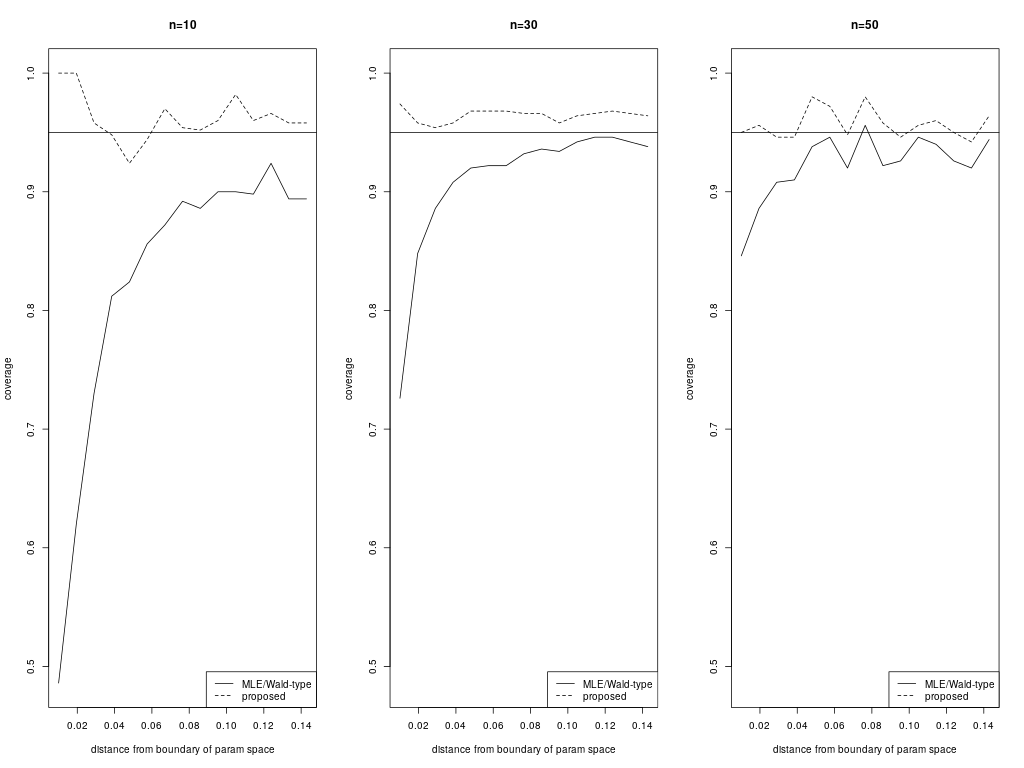
\includegraphics[width=\textwidth]{coverage.png}


\end{document}


could cache the samples from the reference distributions at each
vector p. assumes that the same data set dimensions are being
used. test statistic is being used.

tried sampling from the preimage of theta. intersection of simplex
with a hyperplane.



Do we need exchangeability? 





\message{ !name(manuscript.tex) !offset(-101) }
